\documentclass[]{article}
    %%%%%%%%%%%%%%%%%%%%%%%%%%%%%%%%%%%%%%%%%
% Lachaise Assignment
% Structure Specification File
% Version 1.0 (26/6/2018)
%
% This template originates from:
% http://www.LaTeXTemplates.com
%
% Authors:
% Marion Lachaise & François Févotte
% Vel (vel@LaTeXTemplates.com)
%
% License:
% CC BY-NC-SA 3.0 (http://creativecommons.org/licenses/by-nc-sa/3.0/)
% 
%%%%%%%%%%%%%%%%%%%%%%%%%%%%%%%%%%%%%%%%%

%----------------------------------------------------------------------------------------
%	PACKAGES AND OTHER DOCUMENT CONFIGURATIONS
%----------------------------------------------------------------------------------------

\usepackage{amsmath,amsfonts,stmaryrd,amssymb} % Math packages

\usepackage{enumerate} % Custom item numbers for enumerations

\usepackage[ruled]{algorithm2e} % Algorithms

\usepackage[framemethod=tikz]{mdframed} % Allows defining custom boxed/framed environments

\usepackage{listings} % File listings, with syntax highlighting
\lstset{
	basicstyle=\ttfamily, % Typeset listings in monospace font
}

%----------------------------------------------------------------------------------------
%	DOCUMENT MARGINS
%----------------------------------------------------------------------------------------

\usepackage{geometry} % Required for adjusting page dimensions and margins

\geometry{
	paper=a4paper, % Paper size, change to letterpaper for US letter size
	top=2.5cm, % Top margin
	bottom=3cm, % Bottom margin
	left=2.5cm, % Left margin
	right=2.5cm, % Right margin
	headheight=14pt, % Header height
	footskip=1.5cm, % Space from the bottom margin to the baseline of the footer
	headsep=1.2cm, % Space from the top margin to the baseline of the header
	% showframe, % Uncomment to show how the type block is set on the page
}

%----------------------------------------------------------------------------------------
%	FONTS
%----------------------------------------------------------------------------------------

\usepackage[utf8]{inputenc} % Required for inputting international characters
\usepackage[T1]{fontenc} % Output font encoding for international characters

% \usepackage{XCharter} % Use the XCharter fonts\usepackage{XCharter} % Use the XCharter fonts

%----------------------------------------------------------------------------------------
%	COMMAND LINE ENVIRONMENT
%----------------------------------------------------------------------------------------

% Usage:
% \begin{commandline}
%	\begin{verbatim}
%		$ ls
%		
%		Applications	Desktop	...
%	\end{verbatim}
% \end{commandline}

\mdfdefinestyle{commandline}{
	leftmargin=10pt,
	rightmargin=10pt,
	innerleftmargin=15pt,
	middlelinecolor=black!50!white,
	middlelinewidth=2pt,
	frametitlerule=false,
	backgroundcolor=black!5!white,
	frametitle={Command Line},
	frametitlefont={\normalfont\sffamily\color{white}\hspace{-1em}},
	frametitlebackgroundcolor=black!50!white,
	nobreak,
}

% Define a custom environment for command-line snapshots
\newenvironment{commandline}{
	\medskip
	\begin{mdframed}[style=commandline]
}{
	\end{mdframed}
	\medskip
}

%----------------------------------------------------------------------------------------
%	FILE CONTENTS ENVIRONMENT
%----------------------------------------------------------------------------------------

% Usage:
% \begin{file}[optional filename, defaults to "File"]
%	File contents, for example, with a listings environment
% \end{file}

\mdfdefinestyle{file}{
	innertopmargin=1.6\baselineskip,
	innerbottommargin=0.8\baselineskip,
	topline=false, bottomline=false,
	leftline=false, rightline=false,
	leftmargin=1cm,
	rightmargin=1cm,
	singleextra={%
		\draw[fill=black!10!white](P)++(0,-1.2em)rectangle(P-|O);
		\node[anchor=north west]
		at(P-|O){\ttfamily\mdfilename};
		%
		\def\l{3em}
		\draw(O-|P)++(-\l,0)--++(\l,\l)--(P)--(P-|O)--(O)--cycle;
		\draw(O-|P)++(-\l,0)--++(0,\l)--++(\l,0);
	},
	nobreak,
}

% Define a custom environment for file contents
\newenvironment{file}[1][File]{ % Set the default filename to "File"
	\medskip
	\newcommand{\mdfilename}{#1}
	\begin{mdframed}[style=file]
}{
	\end{mdframed}
	\medskip
}

%----------------------------------------------------------------------------------------
%	NUMBERED QUESTIONS ENVIRONMENT
%----------------------------------------------------------------------------------------

% Usage:
% \begin{question}[optional title]
%	Question contents
% \end{question}

\mdfdefinestyle{question}{
	innertopmargin=1.2\baselineskip,
	innerbottommargin=0.8\baselineskip,
	roundcorner=5pt,
	nobreak,
	singleextra={%
		\draw(P-|O)node[xshift=1em,anchor=west,fill=white,draw,rounded corners=5pt]{%
		Question \theQuestion\questionTitle};
	},
}

\newcounter{Question} % Stores the current question number that gets iterated with each new question

% Define a custom environment for numbered questions
\newenvironment{question}[1][\unskip]{
	\bigskip
	\stepcounter{Question}
	\newcommand{\questionTitle}{~#1}
	\begin{mdframed}[style=question]
}{
	\end{mdframed}
	\medskip
}

%----------------------------------------------------------------------------------------
%	WARNING TEXT ENVIRONMENT
%----------------------------------------------------------------------------------------

% Usage:
% \begin{warn}[optional title, defaults to "Warning:"]
%	Contents
% \end{warn}

\mdfdefinestyle{warning}{
	topline=false, bottomline=false,
	leftline=false, rightline=false,
	nobreak,
	singleextra={%
		\draw(P-|O)++(-0.5em,0)node(tmp1){};
		\draw(P-|O)++(0.5em,0)node(tmp2){};
		\fill[black,rotate around={45:(P-|O)}](tmp1)rectangle(tmp2);
		\node at(P-|O){\color{white}\scriptsize\bf !};
		\draw[very thick](P-|O)++(0,-1em)--(O);%--(O-|P);
	}
}

% Define a custom environment for warning text
\newenvironment{warn}[1][Warning:]{ % Set the default warning to "Warning:"
	\medskip
	\begin{mdframed}[style=warning]
		\noindent{\textbf{#1}}
}{
	\end{mdframed}
}

%----------------------------------------------------------------------------------------
%	INFORMATION ENVIRONMENT
%----------------------------------------------------------------------------------------

% Usage:
% \begin{info}[optional title, defaults to "Info:"]
% 	contents
% 	\end{info}

\mdfdefinestyle{info}{%
	topline=false, bottomline=false,
	leftline=false, rightline=false,
	nobreak,
	singleextra={%
		\fill[black](P-|O)circle[radius=0.4em];
		\node at(P-|O){\color{white}\scriptsize\bf i};
		\draw[very thick](P-|O)++(0,-0.8em)--(O);%--(O-|P);
	}
}

% Define a custom environment for information
\newenvironment{info}[1][Info:]{ % Set the default title to "Info:"
	\medskip
	\begin{mdframed}[style=info]
		\noindent{\textbf{#1}}
}{
	\end{mdframed}
}

    \usepackage{fontspec}
    \usepackage{indentfirst}
    \usepackage{booktabs}
    \usepackage{graphicx}
    \usepackage{subfigure}
    \usepackage{url}
    \setmainfont{思源宋体 CN}
    \XeTeXlinebreaklocale "zh"
    \XeTeXlinebreakskip = 0pt plus 1pt

    \linespread{1.1}

    \title{Computer Vision 2018 Fall Final Project \\ \textbf{超分辨率技术方法综述}}
    \author{张义飞 --- 201821080630\\ \texttt{yidadaa@qq.com}}
    \date{\small{UESTC --- \today}}
    
    \begin{document}

    \maketitle

    \section{超分辨率技术简介}
    超分辨率图像重建 (Super resolution image re-construction, SRIR 或 SR) 是指用信号处理和图像处理的方法 , 通过软件算法的方式将已有的低分辨率 (Low-resolution, LR) 图像转换成高分辨率(High-resolution, HR) 图像的技术 . 它在视频监控(Video surveillance) 、图像打印 (Image printing) 、刑侦分析 (Criminal investigation analysis) 、医学图像处理 (Medical image processing) 、卫星成像(Satellite imaging) 等领域有较广泛的应用。\\

    超分辨率问题的解决涉及到许多图像处理 (Image processing) 、计算机视觉 (Computer vision)、优化理论 (Optimization problem) 等领域中的基本问题, 例如图像配准 (Image registration) 、图像分割 (Image segmentation) 、图像压缩 (Image com-pression) 、图 像 特 征 提 取 (Image feature extraction) 、图像质量评价 (Image quality estimation) 、机器学习 (Machine learning) 、最优化算法 (Optimization algorithm) 等 , 超分辨率是这些基本问题的一个具体应用领域 , 同时也对它们的研究进展起到了推动的作用 . 因此超分辨率问题本身的研究具有重要的理论意义。目前超分辨率问题已经成为相关研究领域的热点之一 .

    \section{超分辨率问题的分类}
    \begin{figure*}[htbp]
        \centering
        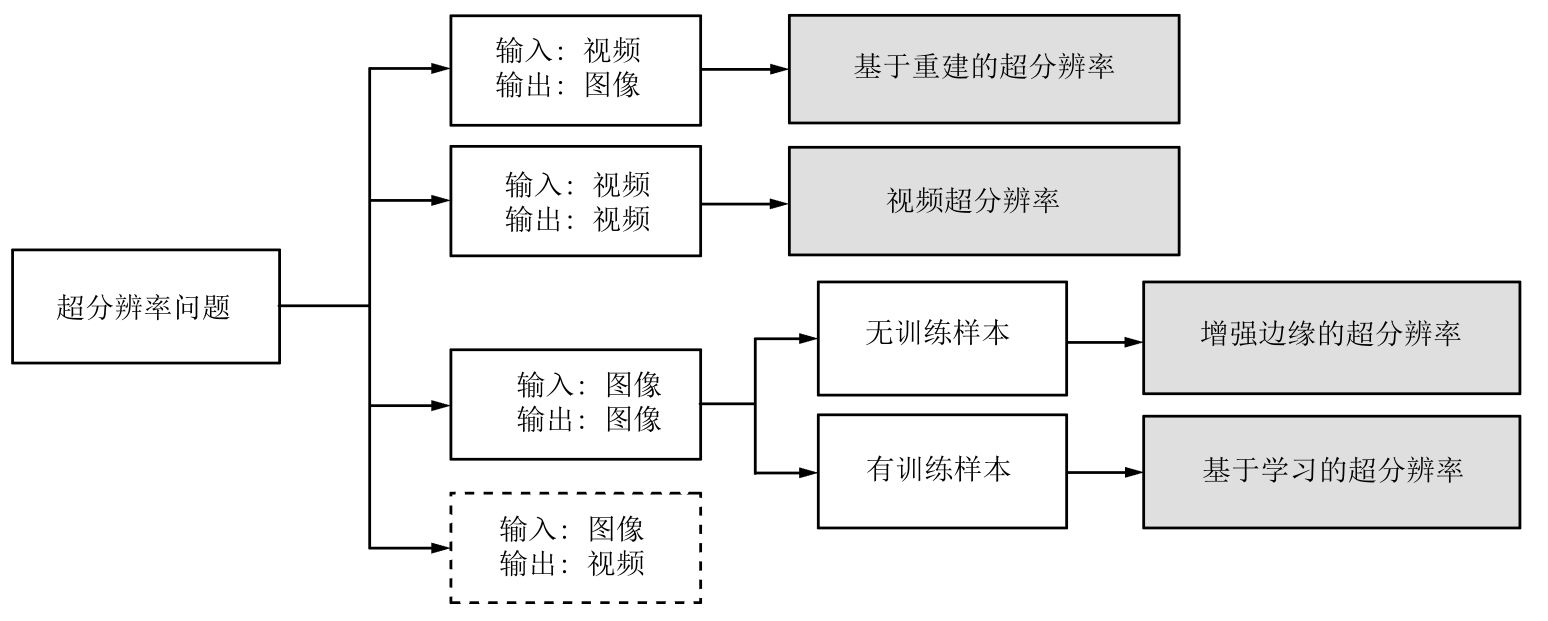
\includegraphics[width=\textwidth]{img/fig-1.png}
        \caption{超分辨率问题的分类}
        \label{fig1}
    \end{figure*}
    概括而言,按算法的输入输出的不同类型组合,超分辨率问题可以分为几类子问题,见图\ref{fig1}。输入为低分辨率图像序列(视频),输出为单帧高分辨率图像的超分辨率问题,称为基于重建的超分辨率问题(Reconstruction-basedsuper-resolution);输入与输出均为图像序列(视频)的超分辨率问题,称为视频超分辨率问题(Videosuper-resolution);输入与输出均为单帧图像的超分辨率问题,称为单帧图像超分辨率问题(Singleimagesuper-resolution,SISR)。\\ 
    
    根据是否依赖训练样本,超分辨率问题又可以分为增强边缘的超分辨率问题(Edge-focusedsuper-resolution)(无训练样本)与基于学习的超分辨率问题(Learning-basedsuper-resolution)(有训练样本)两种。对于输入为单帧低分辨率图像,输出为图像序列(视频)的问题,由于其缺失的信息太多,研究的实际意义不大,几乎没有相关的研究,不在本文的讨论范围之内。以下章节分别综述各种不同类型的超分辨率算法,为了叙述的方便,如果没有特殊说明,用H代表目标高分辨率图像,用$L$代表输入的低分辨率图像,如果输入或输出为图像序列,则用下标$k=1,...,n$来区分不同的图像帧,$n$为总帧数。\\

    \section{基于重建的超分辨率方法}

    基于重建的超分辨率问题是较早提出的一类传统超分辨率问题,首先简单介绍算法常用的数学模型。如图\ref{fig2}所示,假设输入的低分辨率图像共有$n$帧,则基于重建的超分辨率问题的成像模型通常可以表示为:
    \begin{equation}
        L_k=DB^{<2>}_k M_k B^{<1>}_k H+N_k,\ k=1,...,n
    \end{equation}
    模型认为,每一帧观察到的低分辨率图像$L_k$是由未知的原始高分辨率图像$H$经过一系列的图像变换过程得到的,依次为:由环境因素引起的大气模糊算子$B_k^{<1>}$,运动变换算子$M_k$,由相机成像系统引起的成像模糊算子$B_k$(包括运动模糊因素与CCD模糊因素等),以及最后的降采样算子$D$。$N_k$代表在成像过程中引入的加性噪声。已知输入$L_k$,则基于重建的超分辨率的目标就是寻找真实高分辨率图像H的最优估计$\hat H$。
    \begin{figure}[htbp]
        \centering
        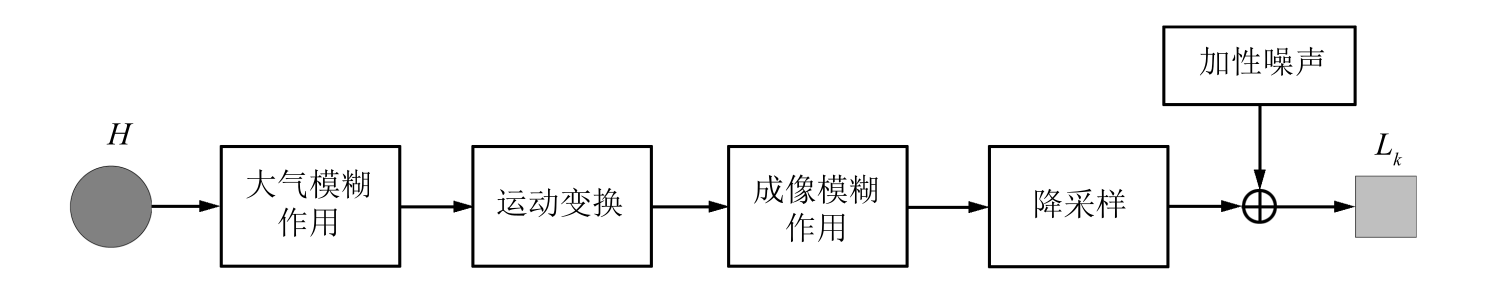
\includegraphics[width=\textwidth]{img/fig-2.png}
        \caption{基于重建的超分辨率问题的常用成像模型}
        \label{fig2}
    \end{figure}

    \section{单帧超分辨率方法}
    前面提到,以单帧图像作为输入的超分辨率问题主要可以分为两类:1)没有训练样本的增强边缘的单帧超分辨率问题;2)有训练样本的基于学习的单帧超分辨率问题。其中,增强边缘的超分辨率问题没有额外信息的辅助,而只是对图像的显示效果(主要是图像边缘)进行增强。因此尽管有一些文献(如文献及最近的文献)将其归入超分辨率的范畴中,严格地说增强边缘的超分辨率并没有从本质上提高图像的分辨率,而应当归类为启发式的(Heuristic)图像增强(Imageenhancement)或图像插值(Imageinterpolation)。\\ 
    
    \begin{figure}[htbp]
        \centering
        \begin{minipage}[t]{0.4\textwidth}
            \centering
            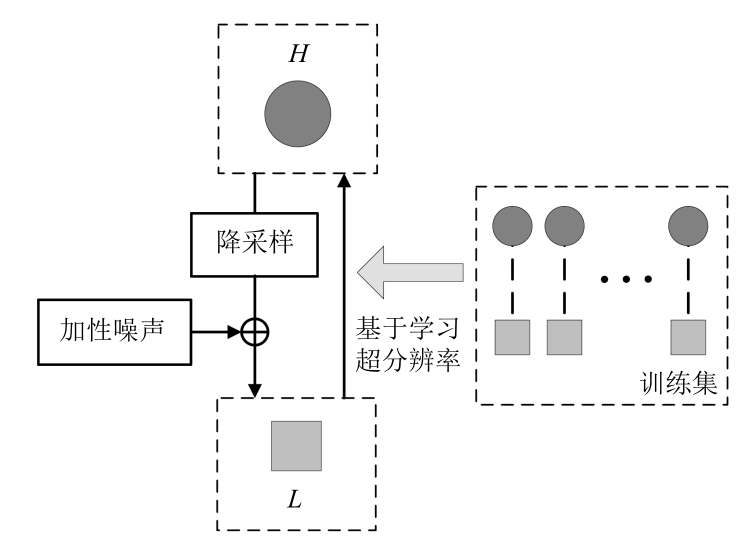
\includegraphics[width=\textwidth]{img/fig-3.png}
        \end{minipage}
        \begin{minipage}[t]{0.4\textwidth}
            \centering
            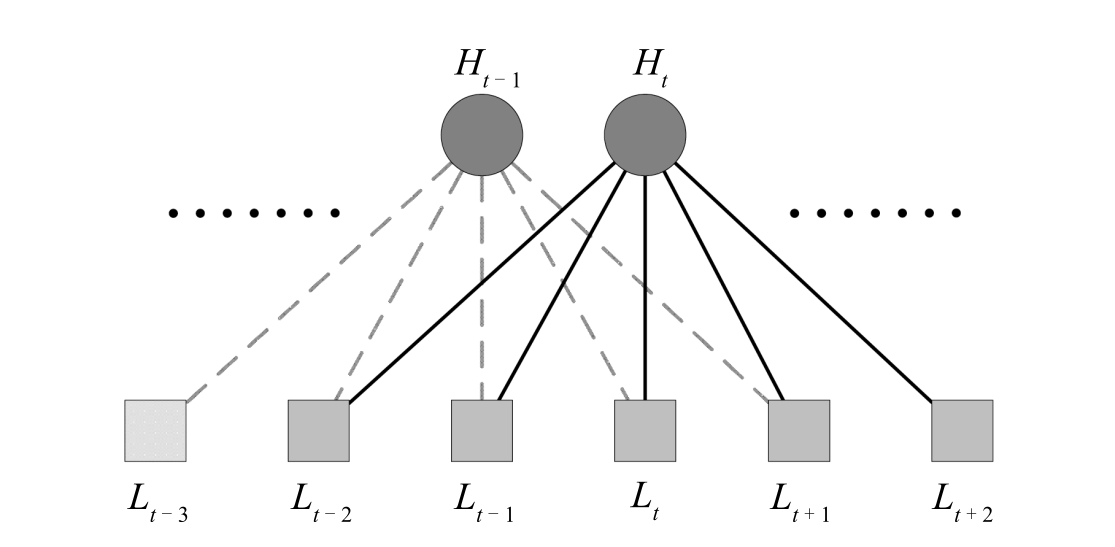
\includegraphics[width=\textwidth]{img/fig-4.png}
        \end{minipage}
        \caption{基于学习的超分辨率问题}
        \label{fig3}
    \end{figure}

    基于学习的单帧超分辨率问题是近年来研究的一个热点,又称为图像幻感(Imagehallucination)或基于样例(Example-based)的超分辨率,它通过机器学习方法从训练样本集中提取所需的高频信息模型,从而对未知测试样本的所需信息进行预测,达到提高图像分辨率的目的,参见图\ref{fig3}。大部分的基于学习的超分辨率方法都是基于分块(Patch-based)的,目标图像平面被分成小的图像块,通过计算求取低分辨率图像块所对应的高分辨率图像块。Pent-land等在1991年提出在训练样本集中进行最近邻搜索以提高压缩图像的质量,是最早采用分块的图像增强方法之一。\\
    
    与基于学习的超分辨率算法相关的核心问题主要有两个部分:算法模型的建立和训练集合的选取。早期(1990年-2005年左右)的相关研究主要着重解决模型建立的问题。文献引入马尔科夫随机场(MRF)来处理包括单帧超分辨率在内的低阶视域(Low-levelvision)任务,在这一工作中考虑了相邻块之间的一致性程度,传统的置信传播算法(Beliefpropagation,BP)被用来进行MRF的概率推断。文献提出在基于学习的超分辨率中使用邻域嵌入(Neighborembedding)更有效地利用训练样本。后来,由于此类算法的运算速度一般较慢,研究者们提出了一系列具有较强针对性的算法,集中对图像中的关键部分进行处理,既可以提高输出质量,又可以减少算法运算时间。文献提出只对图像中的主要区域进行超分辨率化,文献将这些图像中的主要区块提取出来,应用邻域嵌入方法进行超分辨率重建。\\

    随着近几年稀疏表达(Sparserepresentation)的相关理论成为计算机视觉领域的研究热点,基于稀疏表达的超分辨率算法得到了长足发展。Yang等假设输入的低分辨率块可以被训练样本集稀疏线性表达。2010年,Adler等在基于学习的超分辨率中引入了稀疏在线收缩函数(Onlineshrink-agefunction),通过自适应地学习在线收缩函数的形式与系数提高目标图像的分辨率。文献将基于学习的超分辨率问题看作一个回归问题,用稀疏回归(Sparseregression)技术进行快速的回归计算。在模型研究的同时,研究者也开始关注训练样本集的选择与处理,文献提出从训练样本集中学习得到一个更有效的字典(Dictionary)。具有分辨率无关性的图像表达(Resolution-invariantimagerepresentation,RIIR)被应用于快速的多级超分辨率图像重建任务。\\
    
    专门对人脸图像进行基于学习的超分辨率重建的方法也是一个相关的研究热点,可以提高人脸识别的准确度,文献则提出将超分辨率重建与人脸识别这两个过程同时进行,同时得到人脸识别结果与超分辨率化后的人脸图像。最近,文献假设相似的人脸图像具有相似的局部像素结构,从一个已知的人脸数据库中提取信息对输入的低分辨率人脸图像进行超分辨率化。

    \section{总结与展望}
    本文全面地综述了各类超分辨率图像重建算法,并对其进行了比较。作为一个具有很强实用价值的研究领域,超分辨率图像重建具有光明的发展前景,目前超分辨率算法的效果也有着不小的提升空间。在另一方面,我们也应该注意到,提出一个通用而且高效的超分辨率算法比较困难,图像与视频采集设备硬件性能的飞速发展,也会影响到这类通用算法的应用范围。因此,未来的超分辨率算法研究会更多的针对特定具体应用场合,关注实际需求。未来热点的算法研究方向包括:
    \begin{enumerate}
        \item 针对特定应用场合的超分辨率算法。随着智能交通、视频监控、光学文字识别等应用需求的增加,对具体某一类图像的超分辨率算法研究,例如针对人脸、文字、指纹、车牌或其他特定区域的超分辨率算法研究有着重要的意义。在这些专用场合中具有较多的先验知识,将这些先验的知识与超分辨率的算法紧密结合起来,得到的输出图像质量可能会有较大提高。
        \item 与视频编解码算法进行有效结合。以尽量少的码率提供更高质量的视频,对于降低在线视频传输的成本有着非常重要的作用。视频超分辨率与视频压缩的关系非常密切,可以考虑将超分辨率算法与视频编解码算法结合起来,在视频解码的过程中同时进行超分辨率的重建过程,直接提高输出视频的质量。
        \item 基于内容的超分辨率算法。我们进行图像增强的目的通常是主要将感兴趣的部分区域进行重建。因此可以在超分辨率算法中引入对图像内容的识别,进行有针对性的处理。例如,可以首先识别出目标图像中的人脸或文字部分,在相应的部分引入有效的先验信息,提高输出结果质量;或者与图像显著性检测(Imagesaliencydetection)相结合,着重对图像的显著部分进行增强。这种类型的研究,具有较高的实用价值与实际意义。
    \end{enumerate}

    同时,超分辨率图像重建的理论研究涉及到很多与数字图像相关的本质问题,也会是未来的一个热点研究方向。超分辨率重建的理论研究报道目前还比较少,很多相关的问题,包括超分辨率重建的理论极限、图像高低分辨率信息之间的关系等,还属于开放的课题,吸引着研究者进一步的探索。总之,在很长一段时间内,超分辨率图像重建问题将是计算机视觉与图像处理领域的研究热点。更高效的超分辨率算法的提出及超分辨率相关问题的理论突破,都会给这一领域的发展起到重要的推动作用。

    \section{参考文献}
    \begin{enumerate}[(1)]
        \item Capel D, Zisserman A. Computer vision applied to super
        resolution. IEEE Signal Processing Magazine, 2003, 20(3):
        75−86

        \item Tsai R Y, Huang T S. Multiframe image restoration and
        registration. Advances in Computer Vision and Image Pro-
        cessing, 1984, 1: 317−339

        \item Borman S, Stevenson R. Spatial Resolution Enhancement
        of Low-resolution Image Sequences: A Comprehensive Re-
        view with Directions for Future Research, Technical Report,
        Laboratory Image and Signal Analysis, University of Notre
        Dame, 1998

        \item Chaudhuri S. Super-Resolution Imaging. Boston: Kluwer
        Academic Publishers, 2001

        \item Park S C, Park M K, Kan M G. Super-resolution image re-
        construction: a technical overview. IEEE Signal Processing
        Magazine, 2003, 20(3): 21−36

        \item Van Ouwerkerk J D. Image super-resolution survey. Image
        and Vision Computing, 2006, 24(10): 1039−1052

        \item Katartzis A, Petrou M. Current trends in super-resolution
        image reconstruction. Image Fusion: Algorithms and Appli-
        cations. New York: Academic Press, 2008
    \end{enumerate}
    \end{document}